\documentclass[tikz, border=4pt]{standalone}
\usepackage{tikz}
\usepackage{pgf-umlsd}
\begin{document}
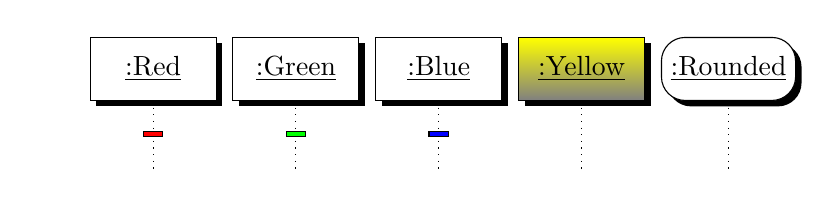
\begin{tikzpicture}[x=1cm, y=1cm]
  \node at (4.36,-0.87) {\pgfinterruptpicture%
  \begin{sequencediagram}
    \newthread[red]{r}{:Red}
    \newthread[green]{g}{:Green}
    \newthread[blue]{b}{:Blue}
    \tikzstyle{inststyle}+=[top color=yellow, bottom color=gray]
    \newinst{y}{:Yellow}
    \tikzstyle{inststyle}+=[bottom color=white, top color=white, rounded corners=3mm]
    \newinst{o}{:Rounded}
  \end{sequencediagram}%
  \endpgfinterruptpicture};
\end{tikzpicture}
\end{document}
